\section{Afstandssensor}

I denne sektion beskrives hvordan ultralydssensoren HC-SR04 er testet for at fastslå hvor pålidelig den er. Testen er udført ved at lave gentagne målinger af afstand mellem ultralyds sensor og en væg. For hver deltest er der foretaget 100 målinger og maksimal værdi, minimal værdi og gennemsnit fundet. 

Ultralydssensoren bruges både til højdemåling og antikollison. Testen bruges til at kontrollere hvorvidt sensoren kan opfylde krav om nøjagtighed til højdemåling\footnote{Se ikke funktionelle krav i \textit{Kravspecifikation}}. 

Undervejs i testen ændres vinklen mellem ultralyds sensor og væg, hvilket indirekte betyder afstande også ændres til væggen. Det formodes at sensoren fungerer bedst når der er en 90 graders vinkel mellem sensor og væg. 

På figur \ref{fig:ultra_testopstilling} vises en skitse af den anvendte testopstilling og tabellen nederst på siden viser resultater af den udførte test.

\begin{figure}[H]
\centering
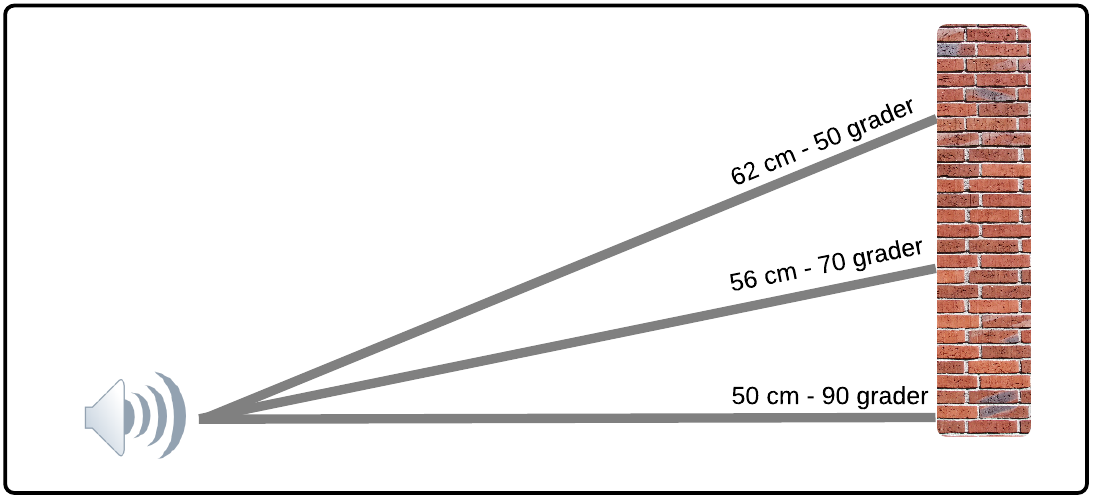
\includegraphics[width=1\textwidth]{Billeder/Test/ultrasound.png}
\caption{Skitse af testopstilling}
\label{fig:ultra_testopstilling}
\end{figure}

\vspace{0.5cm}

\begin{table}[H]
\begin{tabular}{| p{2.5cm}| p{2.5cm}| p{2.5cm}| p{2.5cm}| p{2.5cm}|}
\hline
\textbf{Vinkel} & \textbf{Afstand} & \textbf{Maks måling} & \textbf{Min måling}  & \textbf{Middel værdi} \\ \hline
90 & 50 cm & 49.0 cm & 48.0 cm  & 48.02 cm \\ \hline
70 & 56 cm & 49.0 cm & 49.0 cm  & 49.0 cm \\ \hline
50 & 62 cm & 50.0 cm & 51.0 cm  & 50.0 cm \\ \hline

\end{tabular}
\caption{Test ultralydssensor}
\label{tab:Ultralyds_test}
\end{table}


